% FireForge: a deep dive from the basics.
% Build:  tools/capped latexmk -pdf -outdir=build/guide docs/guide/fireforge-deep-dive.tex
\documentclass[11pt,a4paper]{report}

\usepackage[T1]{fontenc}
\usepackage[utf8]{inputenc}
\usepackage{libertinus}
\usepackage{inconsolata}
\usepackage[margin=2.5cm]{geometry}
\usepackage{microtype}
\usepackage{amsmath,amssymb}
\usepackage{siunitx}
\usepackage{booktabs,tabularx,longtable}
\usepackage{enumitem}
\usepackage{xcolor}
\usepackage{tikz}
\usetikzlibrary{arrows.meta,positioning,fit,calc,shapes.geometric,backgrounds}
\usepackage{pgfplots}
\pgfplotsset{compat=1.18}
\usepackage[most]{tcolorbox}
\usepackage{listings}
\usepackage{titlesec}
\usepackage[hidelinks]{hyperref}

\definecolor{ink}{HTML}{1F2A37}
\definecolor{forge}{HTML}{B4461E}
\definecolor{steel}{HTML}{2F5D8A}
\definecolor{moss}{HTML}{3C7A4A}
\definecolor{paper}{HTML}{F6F4F1}
\definecolor{rule}{HTML}{C9CED6}

\hypersetup{colorlinks=true,linkcolor=steel,urlcolor=steel,citecolor=steel}
\setlist{itemsep=2pt,topsep=4pt}
\setlength{\parskip}{4pt}

\titleformat{\chapter}[display]{\normalfont\bfseries\color{ink}}
  {\large\color{forge}\MakeUppercase{\chaptertitlename}~\thechapter}{4pt}{\Huge}
\titlespacing*{\chapter}{0pt}{-20pt}{24pt}
\titleformat{\section}{\normalfont\Large\bfseries\color{ink}}{\thesection}{0.8em}{}
\titleformat{\subsection}{\normalfont\large\bfseries\color{ink}}{\thesubsection}{0.8em}{}

\newtcolorbox{keyidea}[1][Key idea]{enhanced,breakable,colback=paper,colframe=forge,
  boxrule=0pt,leftrule=3pt,arc=0pt,fonttitle=\bfseries\color{forge},coltitle=forge,
  colbacktitle=paper,title=#1,attach title to upper={\ \ },left=8pt}
\newtcolorbox{inff}[1][In FireForge]{enhanced,breakable,colback=steel!6,colframe=steel,
  boxrule=0pt,leftrule=3pt,arc=0pt,fonttitle=\bfseries,coltitle=steel,
  colbacktitle=steel!6,title=#1,attach title to upper={\ \ },left=8pt}

\lstset{basicstyle=\ttfamily\small,columns=fullflexible,keepspaces=true,
  backgroundcolor=\color{paper},frame=none,xleftmargin=6pt,xrightmargin=6pt,
  aboveskip=6pt,belowskip=6pt,breaklines=true,showstringspaces=false}

\newcommand{\code}[1]{\texttt{#1}}
\newcommand{\kl}{\kappa_\mathrm{l}}
\newcommand{\ke}{\kappa_\mathrm{e}}

\tikzset{
  box/.style={draw=ink,rounded corners=2pt,fill=white,align=center,inner sep=5pt,font=\small},
  sbox/.style={box,fill=steel!8,draw=steel},
  fbox/.style={box,fill=forge!8,draw=forge},
  mbox/.style={box,fill=moss!10,draw=moss},
  arr/.style={-{Stealth[length=2.2mm]},thick,draw=ink!80},
  darr/.style={arr,dashed},
  lab/.style={font=\scriptsize,text=ink!80},
}

\title{\vspace*{-2cm}{\color{forge}\rule{\linewidth}{2pt}}\\[10pt]
  {\Huge\bfseries FireForge}\\[6pt]
  {\Large A deep dive from the basics}\\[4pt]
  {\large physics, computation and the distributed system}\\
  {\color{forge}\rule{\linewidth}{1pt}}}
\author{Written for the FireForge team}
\date{November 2026, describing Phases 1--9}

\begin{document}
\maketitle

\begin{abstract}
FireForge is a platform for discovering new materials by computer. It predicts how well a
crystal would turn heat into electricity, starting from nothing but the positions of its
atoms, and does this for many candidates at once on a small cluster of Linux machines.
This guide explains the whole thing from first principles: the physics of thermoelectrics,
how quantum-mechanical simulation works, what each calculation in the pipeline computes,
and how the distributed runtime moves the work and the data between machines. It ends by
following one compound, ZrNiSn, through the running system. No background beyond
school physics and basic programming is assumed.
\end{abstract}

\tableofcontents

%======================================================================
\part{The big picture}
%======================================================================

\chapter{What FireForge is for}

\section{The problem: finding materials by computation}

Every technology is limited by its materials. Batteries are limited by electrodes, solar
cells by absorbers, engines by alloys that survive heat. Finding a better material by
experiment is slow: you have to guess a composition, synthesise it, grow a clean sample and
measure it, which can take months for one compound. The number of possible compounds is
astronomically larger than anyone could make.

Since the 1990s, physics and computing have reached the point where many material
properties can be \emph{predicted} from quantum mechanics before anyone makes the material.
The input is only which atoms are present and where they sit. The output is energies,
electronic band structures, vibrations, conductivities and stabilities. Each prediction
costs minutes to days of computer time instead of months of lab time, and many can run in
parallel. That turns discovery into a search problem: generate candidates, compute their
properties, rank them, and send only the best few to an experimental lab.

FireForge is built to run that search. Its first target is \textbf{thermoelectric
materials}, which convert a temperature difference directly into electric power (and the
reverse, for solid-state cooling).

\section{Two halves}

FireForge has two parts that you can understand separately.

\begin{description}
\item[The science suite] (\code{science/fireforge\_science}). Python code that knows the
  physics: how to build candidate crystals, drive the quantum-mechanics solver (Quantum
  ESPRESSO), compute vibrations (Phonopy, phono3py), compute electrical transport
  (BoltzTraP2), check stability, and combine everything into a thermoelectric figure of
  merit, $ZT$. It is organised in modules named CrystalForge, QuantumForge, PhonoForge,
  TransportForge and StabilityForge.
\item[TDR, the distributed runtime] (\code{runtime/}, \code{control/}). C++ infrastructure
  that runs the science code as \emph{jobs} on many machines. It decides which machine runs
  what, enforces CPU and memory limits, moves result files between machines, retries work
  when a machine dies, and records every result in a database. It knows nothing about
  physics.
\end{description}

The science code is written as \emph{workers}: small programs that receive one task
(``relax this crystal''), do it, and hand back files and records. TDR treats a worker like
any other program. This separation means the physics can change without touching the
distributed system, and the runtime could run any other kind of scientific code.

\section{The machines in this deployment}

\begin{figure}[h]
\centering
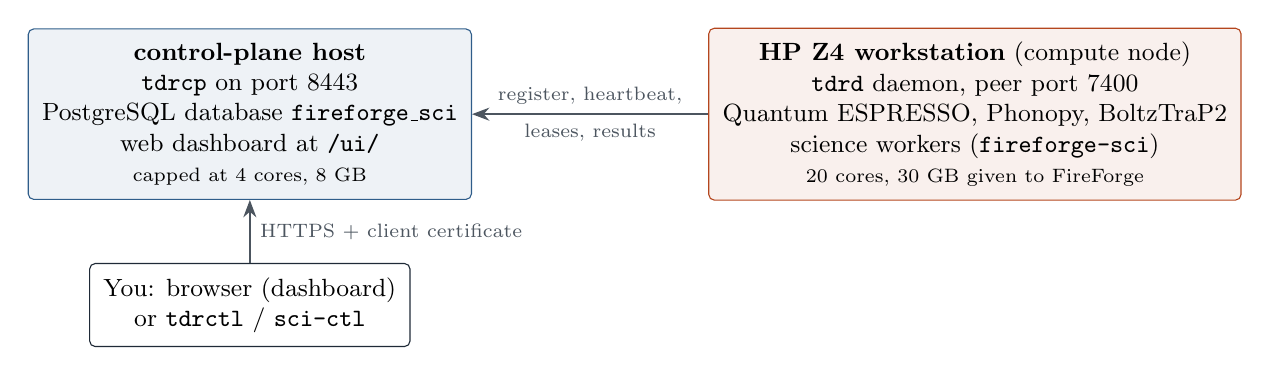
\begin{tikzpicture}[node distance=8mm and 30mm]
\node[sbox,minimum width=4.6cm] (cp) {\textbf{control-plane host}\\
  \code{tdrcp} on port 8443\\ PostgreSQL database \code{fireforge\_sci}\\
  web dashboard at \code{/ui/}\\ \scriptsize capped at 4 cores, 8 GB};
\node[fbox,minimum width=4.6cm,right=of cp] (hp) {\textbf{HP Z4 workstation} (compute node)\\
  \code{tdrd} daemon, peer port 7400\\ Quantum ESPRESSO, Phonopy, BoltzTraP2\\
  science workers (\code{fireforge-sci})\\ \scriptsize 20 cores, 30 GB given to FireForge};
\node[box,below=of cp] (you) {You: browser (dashboard)\\ or \code{tdrctl} / \code{sci-ctl}};
\draw[arr] (hp.west) -- node[above,lab]{register, heartbeat,} node[below,lab]{leases, results} (cp.east);
\draw[arr] (you) -- node[right,lab]{HTTPS + client certificate} (cp);
\end{tikzpicture}
\caption{The deployment running the Phase 8 validation. Both machines talk over Tailscale
(the \code{100.x.y.z} addresses).}
\label{fig:deploy}
\end{figure}

The \textbf{control plane} is the coordinator. It holds the job queue, the workflow state
and the materials database, but runs no science itself. The \textbf{compute node} does the
calculations. More nodes can join at any time: they register, advertise what software they
have, and start pulling work. Running jobs never depend on the control plane being up; if
it restarts, nodes keep computing and reconnect.

\section{How to read this guide}

Part~II builds the physics from the ground up, ending with exactly what each step of the
pipeline computes. Part~III explains the distributed system, phase by phase, in the order
it was built. Part~IV follows one compound through the live system and lists the practical
commands. A glossary is at the end. You can read Part~III before Part~II if you are more
interested in the software.

%======================================================================
\part{The physics}
%======================================================================

\chapter{Crystals}

\section{Atoms in a repeating pattern}

A crystal is a solid whose atoms sit in a pattern that repeats in all three directions.
Because it repeats, you only need to describe one tile, the \textbf{unit cell}, and how it
is stacked. The unit cell is a parallelepiped spanned by three \textbf{lattice vectors}
$\mathbf a_1,\mathbf a_2,\mathbf a_3$. Every atom position can be written in
\textbf{fractional coordinates} $(x,y,z)$, meaning the point
$x\,\mathbf a_1+y\,\mathbf a_2+z\,\mathbf a_3$, with $0\le x,y,z<1$ inside the cell.

That is exactly how FireForge stores a structure: nine numbers for the lattice (three
vectors in \si{\angstrom}; $\SI{1}{\angstrom}=10^{-10}\,\mathrm{m}$, roughly the size of an
atom) and a list of sites, each a chemical species with three fractional coordinates.

\begin{inff}
A real record from the database, ZrNiSn after relaxation (rounded):
\begin{lstlisting}
lattice: [0, 3.044, 3.044,   3.044, 0, 3.044,   3.044, 3.044, 0]   (Angstrom)
sites:   Zr (0, 0, 0)   Ni (0.25, 0.25, 0.25)   Sn (0.5, 0.5, 0.5)
spacegroup F-43m (216), prototype half-heusler
\end{lstlisting}
Three atoms in the smallest (primitive) cell. The lattice vectors are the face-centred
cubic ones, $\tfrac a2(0,1,1)$, $\tfrac a2(1,0,1)$, $\tfrac a2(1,1,0)$, with
$a=2\times3.044=\SI{6.088}{\angstrom}$ here. The conventional cubic cell with edge $a$ holds four of these.
\end{inff}

\section{Symmetry and space groups}

Crystals have symmetry: rotations, mirrors and translations that map the pattern onto
itself. Every crystal belongs to one of 230 \textbf{space groups}. Symmetry matters for two
practical reasons. First, it reduces work: symmetric points need to be computed only once.
Second, it gives a robust way to tell whether two structure descriptions are really the same
crystal (shifted, rotated, or with atoms listed in another order).

FireForge uses the \code{spglib} library to find the symmetry and reduce every structure to a
standard form. It then hashes that standard form into a \textbf{fingerprint}
(\code{fp1:} followed by a SHA-256 hash). Two structures with the same fingerprint are the same
crystal, so the database stores it once. A relaxed structure is a new structure that points
back to its parent.

\section{The half-Heusler family}

The first campaign studies \textbf{half-Heusler} compounds, written $XYZ$: one transition
metal $X$ (e.g.\ Zr, Hf, Ti, Nb), one late transition metal $Y$ (Ni, Co, Fe), and one main-group
element $Z$ (Sn, Sb). They are among the best-studied thermoelectrics at high temperature, are
made of relatively cheap elements, and are mechanically tough.

All half-Heuslers share space group $F\bar43m$ (number 216). Picture four interpenetrating
face-centred cubic lattices placed along the cube's body diagonal at $0$, $\tfrac14$,
$\tfrac12$ and $\tfrac34$ of the way. In a half-Heusler three of the four are occupied and one
is empty (a full Heusler $XY_2Z$ fills all four):

\begin{center}
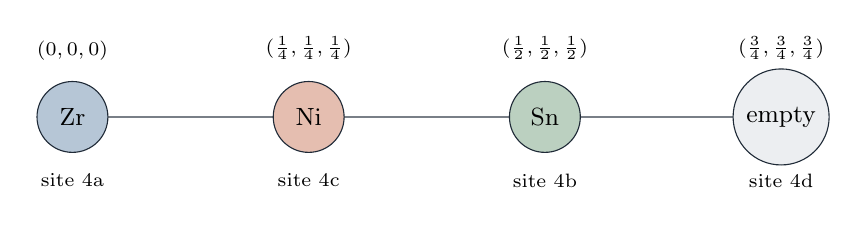
\begin{tikzpicture}[x=3cm]
\draw[thick,ink!60] (0,0) -- (3,0);
\foreach \p/\lbl/\site/\col in {0/Zr/4a/steel, 1/Ni/4c/forge, 2/Sn/4b/moss, 3/empty/4d/rule}{
  \node[circle,draw=ink,fill=\col!35,minimum size=9mm] at (\p,0) {\small\lbl};
  \node[below=6mm,font=\scriptsize] at (\p,0) {site \site};
}
\foreach \p/\f in {0/0,1/{\tfrac14},2/{\tfrac12},3/{\tfrac34}}{
  \node[above=6mm,font=\scriptsize] at (\p,0) {$(\f,\f,\f)$};
}
\end{tikzpicture}
\end{center}

Which element sits on the special site 4c (between the other two) changes the compound. For
three elements there are three distinct \textbf{orderings}. Known half-Heuslers put the late
transition metal $Y$ on 4c, and FireForge's campaign builder tries all three and keeps the one
with lowest energy.

\begin{keyidea}[The 18-electron rule]
Half-Heuslers with 8 or 18 valence electrons per formula unit tend to be semiconductors,
which is what a thermoelectric needs. ZrNiSn: Zr 4 + Ni 10 + Sn 4 = 18. NbFeSb: 5 + 8 + 5 = 18.
The candidate generator \code{crystal.halfheusler} uses this count (parameter
\code{electron\_counts} = [8, 18]) to discard compositions that are probably metals.
\end{keyidea}

The five compounds in the validation set are ZrNiSn, HfNiSn, TiNiSn, NbFeSb and ZrCoSb. They
are all well characterised experimentally, so the predictions can be checked.

\chapter{Thermoelectrics}

\section{The Seebeck effect}

Heat one end of a conductor and cool the other. The mobile charge carriers (electrons or
holes) on the hot side have more kinetic energy and diffuse towards the cold side faster than
the cold ones diffuse back. Charge piles up at the cold end until the resulting electric field
stops the net flow. The voltage this creates is proportional to the temperature difference:
\begin{equation}
  V = S\,\Delta T,
\end{equation}
where $S$ is the \textbf{Seebeck coefficient}, measured in \si{\micro\volt\per\kelvin}. For
metals $S$ is a few \si{\micro\volt\per\kelvin}; for good thermoelectric semiconductors it is
150--250\,\si{\micro\volt\per\kelvin}. Its sign tells you the carrier type: negative for
electrons (\textbf{n-type}), positive for holes (\textbf{p-type}). A thermoelectric generator
connects n- and p-type legs electrically in series and thermally in parallel.

\section{The figure of merit $ZT$}

How efficiently a material converts heat to electricity is summarised by one dimensionless
number,
\begin{equation}
  ZT = \frac{S^2\sigma\,T}{\ke+\kl},
\end{equation}
with $\sigma$ the electrical conductivity, $T$ the absolute temperature, and $\kappa$ the thermal
conductivity, split into the part carried by the electrons ($\ke$) and the part carried by
lattice vibrations ($\kl$). The numerator $S^2\sigma$ is the \textbf{power factor} (PF,
reported in \si{\micro\watt\per\centi\metre\per\kelvin\squared}). Commercial materials reach
$ZT\approx1$; $ZT$ above 2 would make waste-heat recovery widely practical.

\section{Why high $ZT$ is hard}

Each quantity pulls against another.

\begin{itemize}
\item More carriers raise $\sigma$ but lower $S$. Metals conduct well but have tiny $S$;
  insulators have huge $S$ but do not conduct. The power factor peaks in heavily doped
  semiconductors, near $10^{19}$--$10^{21}$ carriers per \si{\centi\metre\cubed}
  (Figure~\ref{fig:tradeoff}).
\item The electrons that carry charge also carry heat. The Wiedemann--Franz law ties them
  together: $\ke = L\sigma T$, with $L$ the Lorenz number. You cannot raise $\sigma$ without
  raising $\ke$.
\item That leaves $\kl$ as the one quantity you can lower almost independently. Heavy atoms,
  complex unit cells, strong anharmonicity (non-spring-like bonds) and disorder all scatter
  vibrations and lower $\kl$. This is why FireForge spends so much effort computing $\kl$.
\end{itemize}

\begin{figure}[h]
\centering
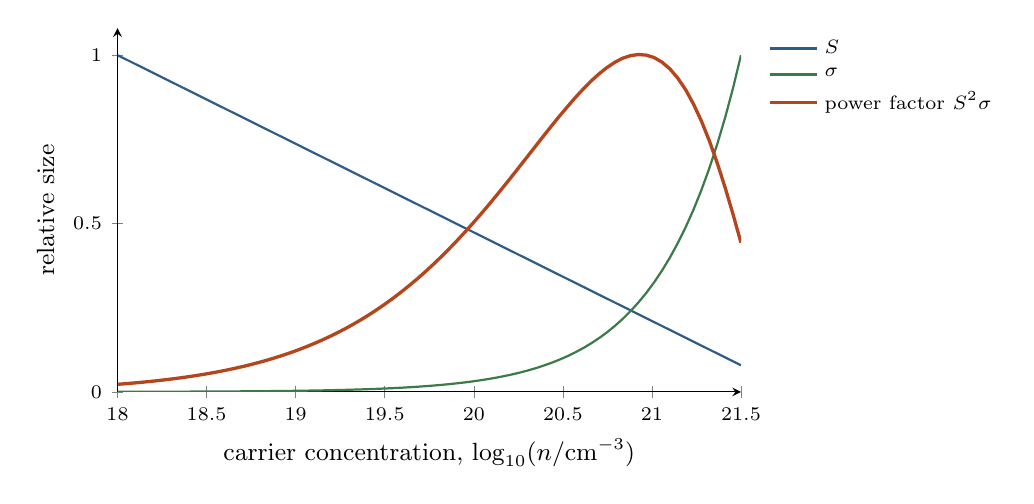
\begin{tikzpicture}
\begin{axis}[width=9.5cm,height=6.2cm,domain=18:21.5,samples=80,
  xlabel={carrier concentration, $\log_{10}(n/\mathrm{cm}^{-3})$},ylabel={relative size},
  ymin=0,ymax=1.08,xmin=18,xmax=21.5,legend pos=outer north east,legend cell align=left,legend style={font=\scriptsize,draw=none,fill=none},
  ticklabel style={font=\scriptsize},label style={font=\small},axis lines=left]
\addplot[thick,steel] {(21.8-x)/3.8};                       \addlegendentry{$S$}
\addplot[thick,moss] {10^(x-21.5)};                         \addlegendentry{$\sigma$}
\addplot[very thick,forge] {((21.8-x)/3.8)^2*10^(x-21.5)/0.01408}; \addlegendentry{power factor $S^2\sigma$}
\end{axis}
\end{tikzpicture}
\caption{Schematic trade-off with doping. $S$ falls and $\sigma$ rises with carrier
concentration, so the power factor has a maximum. Real curves come from the transport
calculation (Chapter~\ref{ch:transport}).}
\label{fig:tradeoff}
\end{figure}

\section{Temperature regimes}

$ZT$ depends strongly on temperature, and different applications run at different
temperatures. FireForge reports $ZT$ averaged over four windows:

\begin{center}
\begin{tabular}{lll}
\toprule
Regime & Range & Example use \\
\midrule
low & 300--500\,K & body heat, electronics cooling \\
intermediate & 500--800\,K & industrial waste heat, car exhaust \\
high & 800--1100\,K & furnaces; half-Heuslers peak here \\
extreme & above 1100\,K & space power (radioisotope generators) \\
\bottomrule
\end{tabular}
\end{center}

\section{What a good candidate needs}

$ZT$ alone is not enough. A useful material must also be:
\begin{itemize}
\item \textbf{thermodynamically stable}: it should not decompose into other compounds;
\item \textbf{dynamically stable}: its atoms should sit at a true energy minimum, not a saddle;
\item \textbf{mechanically stable}: it should resist shear and compression;
\item a \textbf{semiconductor} with a band gap, so it can be doped to the right carrier density;
\item made of \textbf{abundant, affordable, non-toxic} elements.
\end{itemize}
Each of these becomes a calculation in the pipeline. The rest of Part~II explains them.

\chapter{Quantum mechanics on a computer: DFT}
\label{ch:dft}

\section{Why quantum mechanics}

The properties above are all determined by how electrons arrange themselves around the
nuclei. Electrons obey quantum mechanics: their behaviour is described by a wavefunction
satisfying the Schrödinger equation. For a crystal with $10^{23}$ interacting electrons the
exact equation is hopeless. The workhorse approximation that makes it tractable is
\textbf{density functional theory} (DFT), which earned Walter Kohn a Nobel Prize in 1998 and is
now used in tens of thousands of papers a year.

\section{The idea of DFT}

DFT rests on a theorem: the ground-state energy of the electrons is a functional of the
\emph{electron density} $n(\mathbf r)$ alone, a function of three coordinates instead of
$3N$. Kohn and Sham turned this into a practical scheme. They replace the real interacting
electrons with fictitious non-interacting ones moving in an effective potential chosen so that
they have the same density. Each fictitious electron obeys a one-particle equation,
\begin{equation}
  \Bigl[-\tfrac{\hbar^2}{2m}\nabla^2 + V_\mathrm{nuclei}(\mathbf r) + V_\mathrm{H}[n](\mathbf r)
  + V_\mathrm{xc}[n](\mathbf r)\Bigr]\psi_i(\mathbf r) = \varepsilon_i\,\psi_i(\mathbf r),
  \qquad n(\mathbf r)=\sum_i^{\text{occupied}}|\psi_i(\mathbf r)|^2 .
\end{equation}
$V_\mathrm{H}$ is the classical electrostatic repulsion of the density, and $V_\mathrm{xc}$,
the \textbf{exchange--correlation} potential, contains all the hard many-body quantum effects.
Its exact form is unknown and must be approximated.

\begin{keyidea}[The self-consistent loop (SCF)]
The potential depends on the density, and the density depends on the solutions. So DFT codes
iterate: guess a density, build the potential, solve for the orbitals, compute a new density,
mix it with the old one, and repeat until nothing changes (to a tolerance such as
$10^{-8}$\,Ry in energy). This is the ``SCF'' in \code{qe.scf}.
\end{keyidea}

\section{The approximations you will see in the records}

Every calculation record stores its \code{method}, which lists the choices below. They matter
for interpreting results.

\begin{description}
\item[Functional: PBE.] FireForge uses the Perdew--Burke--Ernzerhof generalised-gradient
  approximation for $V_\mathrm{xc}$. PBE is the standard for solids. Its known biases:
  lattice constants come out about 1\% too large, and \textbf{band gaps come out too small},
  often by 30--50\%. This is why validation compares predicted gaps with \emph{published PBE}
  gaps, not with measured ones.
\item[Pseudopotentials: SSSP.] Core electrons, close to the nucleus, barely take part in
  bonding but are expensive to describe. Pseudopotentials replace the nucleus plus core
  electrons with a smooth effective potential. FireForge uses the curated SSSP~1.3 ``PBE
  efficiency'' library, downloaded and checksum-verified by \code{tools/sci-setup.sh}. Each
  record lists the files and their MD5 checksums, so results are reproducible.
\item[Plane-wave cutoff.] In a periodic crystal it is natural to expand orbitals in plane
  waves $e^{i\mathbf G\cdot\mathbf r}$. Precision is controlled by the maximum kinetic energy
  included, the cutoff (in Ry). SSSP recommends a cutoff per element; FireForge uses the largest
  among the elements present, multiplied by 1.25 in the \code{accurate} preset.
\item[k-points.] Electrons in a crystal are labelled by a wave vector $\mathbf k$ in the
  \textbf{Brillouin zone}. Integrals over $\mathbf k$ are done on a grid. FireForge sets the
  grid by a target spacing (the ASE \code{kspacing} convention), so denser grids for small
  cells and coarser ones for big supercells.
\end{description}

\section{Quantum ESPRESSO and \code{pw.x}}

FireForge uses Quantum ESPRESSO (QE) 6.7, an open-source DFT package; its main program is
\code{pw.x}. FireForge writes an input file, runs
\code{mpirun -np \textit{cpus} pw.x -in pw.in}, and parses the output files. Three kinds of runs
matter:

\begin{description}
\item[Relaxation (\code{qe.relax}).] Atoms and the cell shape move downhill in energy until the
  forces on atoms and the stress on the cell vanish (a ``vc-relax'', variable-cell relaxation).
  Output: the equilibrium structure and its total energy. Everything else is computed on this
  relaxed structure, because properties at the wrong lattice constant are meaningless.
\item[Self-consistent run (\code{qe.scf}).] Solves the SCF loop on a normal $k$ grid and saves the
  converged density and potential.
\item[Non-self-consistent run (\code{qe.nscf}).] Reuses the saved potential and solves for the
  orbital energies on a much denser $k$ grid, without iterating. This gives the
  \textbf{band structure} $\varepsilon_n(\mathbf k)$ in fine detail, which transport needs.
\end{description}

\section{Bands and the band gap}

The orbital energies $\varepsilon_n(\mathbf k)$ form bands. At zero temperature electrons fill
bands up to the Fermi level. In a semiconductor the last filled band (valence band) and first
empty band (conduction band) are separated by a \textbf{band gap}. The top of the valence band
(VBM) and bottom of the conduction band (CBM) can sit at the same $\mathbf k$ (\textbf{direct}
gap) or at different ones (\textbf{indirect}). The \code{qe.bands} record stores the gap, its
character, VBM, CBM and electron count.

\begin{inff}[In FireForge: the first real result]
The ZrNiSn screening relaxation on the HP workstation took 591\,s on 4 cores and gave
$a=\SI{6.150}{\angstrom}$. The measured value is \SI{6.110}{\angstrom}, 0.7\% smaller, as
expected for PBE. Validation allows 2\%.
\end{inff}

\chapter{Vibrations: phonons and thermal conductivity}

\section{Atoms on springs}

Atoms in a crystal are not frozen; they vibrate about their equilibrium positions. For small
displacements the energy rises quadratically, as if neighbouring atoms were joined by springs
(the \textbf{harmonic approximation}). The ``spring constants'' are the \textbf{second-order
force constants} $\Phi_{ij}=\partial^2E/\partial u_i\partial u_j$. Because the crystal repeats,
collective vibrations are waves, and quantised vibrational waves are called \textbf{phonons}.
Each wave vector $\mathbf q$ has $3N$ phonon modes for $N$ atoms per cell: three
\emph{acoustic} modes (sound waves) and $3N-3$ \emph{optical} ones. Phonons carry heat, and
that heat flow is $\kl$.

\section{Computing force constants: finite displacements}

FireForge computes force constants the direct way, using Phonopy:
\begin{enumerate}
\item Build a \textbf{supercell}, the unit cell repeated a few times in each direction, so that a
  displaced atom does not interact with its own periodic copies.
\item Displace one atom by a tiny amount (about \SI{0.01}{\angstrom}). Symmetry means only a few
  displacements are needed.
\item Run DFT on each displaced supercell and read the forces on all atoms
  (\code{qe.forces}).
\item From force $=-\Phi\times$ displacement, fit $\Phi$. Diagonalising the
  \emph{dynamical matrix} built from $\Phi$ gives the phonon frequencies at any $\mathbf q$.
\end{enumerate}

Each displaced supercell is an independent DFT run, so they can run in parallel on different
cores or machines. That is why \code{phonon.harmonic} does not compute anything itself: it
\emph{spawns} one \code{qe.forces} job per supercell plus a \code{phonon.collect} job to fit the
results (the ``$\times10$'' boxes in the dashboard's step graph).

\begin{keyidea}[Imaginary frequencies mean instability]
If the energy goes \emph{down} along some displacement, the ``spring constant'' is negative and
the frequency comes out imaginary (shown as negative, in THz). The structure is then not at a
minimum and would distort. \code{phonon.harmonic} records \code{min\_freq\_thz} and
\code{dynamically\_stable}; unstable candidates are rejected.
\end{keyidea}

\section{Anharmonicity and the Grüneisen parameter}

Perfect springs would let phonons pass through each other forever, giving infinite thermal
conductivity. Real bonds are \emph{anharmonic}: stiffness depends on how stretched they are,
and this lets phonons scatter off each other. A simple measure is the \textbf{Grüneisen
parameter} $\gamma=-\partial\ln\omega/\partial\ln V$: how much frequencies shift when the crystal
is squeezed. FireForge repeats the phonon calculation at three volumes (strains of $-2\%$, $0$ and
$+2\%$, the \textbf{quasi-harmonic} approach) and averages $\gamma$ over the acoustic modes. Large
$\gamma$ means strong scattering and low $\kl$.

\section{Tier 1: the Slack model}

Computing $\kl$ exactly is expensive, so FireForge first uses a well-tested formula, the
\textbf{Slack model}:
\begin{equation}
  \kl = A(\gamma)\,\frac{\bar M\,\theta_a^3\,\delta\,n^{1/3}}{\gamma^2\,T},
  \qquad A(\gamma)=\frac{2.43\times10^{-8}}{1-0.514/\gamma+0.228/\gamma^2},
\end{equation}
with $\bar M$ the average atomic mass (amu), $\delta^3$ the volume per atom
(\si{\angstrom\cubed}), $n$ the number of atoms per primitive cell, $\theta_a=\theta_D n^{-1/3}$ the
acoustic Debye temperature (K) and $A(\gamma)$ Julian's prefactor. The Debye temperature
$\theta_D$ comes from the phonon density of states. The model captures the main trends
(heavy atoms, low $\theta_D$ and large $\gamma$ give low $\kl$, and $\kl\propto1/T$) but is only
accurate to about a factor of two. The \code{phonon.slack} record stores $\kl$ at 300, 500, 800
and 1100\,K.

\section{Tier 2: phono3py and the Boltzmann equation}

For promising candidates FireForge runs the expensive method. It computes
\textbf{third-order force constants} (how the force on one atom depends on displacements of two
others) by displacing \emph{pairs} of atoms, which takes hundreds of DFT force calculations. With
these, phono3py computes every phonon--phonon scattering rate and solves the phonon
\textbf{Boltzmann transport equation} in the relaxation-time approximation. The result
(\code{phonon.bte}) is typically within 20--30\% of experiment for clean crystals.

\begin{inff}
\code{te.evaluate} spawns this tier automatically when a candidate passes screening
(\code{tier2: auto}). In the validation workflow it is forced for ZrNiSn and turned off for the
other four to bound runtime: the third-order calculation is the single most expensive part of
the run.
\end{inff}

\chapter{Electrons in motion: transport}
\label{ch:transport}

\section{The Boltzmann picture}

To get $S$, $\sigma$ and $\ke$, think of electrons as particles with velocity
$\mathbf v_n(\mathbf k)=\hbar^{-1}\nabla_{\mathbf k}\varepsilon_n(\mathbf k)$, taken directly from the
band structure. An electric field or temperature gradient pushes the electron distribution
slightly out of equilibrium; scattering (off phonons, impurities, defects) pulls it back over a
characteristic \textbf{relaxation time} $\tau$. The electronic Boltzmann equation, linearised,
gives all three coefficients as integrals over the bands weighted by velocities, $\tau$, and
derivatives of the Fermi--Dirac distribution.

\section{The constant relaxation time approximation}

Computing $\tau$ from first principles is very expensive. The standard shortcut, used here, is
the \textbf{constant relaxation time approximation} (CRTA): take $\tau$ to be the same for all
electrons. Then:
\begin{itemize}
\item $S$ does not depend on $\tau$ at all. It is a genuine prediction.
\item $\sigma$ and $\ke$ are proportional to $\tau$. The code computes $\sigma/\tau$, and a value
  for $\tau$ must be assumed. FireForge uses $\tau=10^{-14}$\,s, typical for these materials.
\end{itemize}
So $ZT$ values depend on the assumed $\tau$ and should be read as estimates for ranking, not
absolute predictions. Every record states the $\tau$ it assumed (\code{tau\_s}) and flags it
in its uncertainty field.

\section{BoltzTraP2}

The transport integrals need band velocities on a very fine $k$ grid. BoltzTraP2 interpolates
the DFT bands from the \code{qe.nscf} grid with smooth Fourier functions and evaluates the
integrals. FireForge scans temperatures from 300 to 1200\,K and doping levels from $10^{18}$ to
$10^{21}$\,cm$^{-3}$ for both electrons and holes (\code{transport.boltztrap}). Doping is modelled
by shifting the chemical potential, assuming the bands do not change (``rigid band'').

\section{Putting $ZT$ together}

\code{te.evaluate} combines, at every temperature and doping level,
$S$, $\sigma$ and $\ke$ from transport with $\kl$ from phonons:
\[
  ZT(T,n) = \frac{S(T,n)^2\,\sigma(T,n)\,T}{\ke(T,n)+\kl(T)} .
\]
For each temperature it takes the best doping, separately for p- and n-type, and reports the
peak $ZT$, the temperature and doping where it occurs, regime averages, and the curves the
dashboard plots.

\chapter{Stability}

\section{Thermodynamic: formation energy and the convex hull}

A compound is only useful if it does not prefer to break into something else. The
\textbf{formation energy} per atom compares it with its elements in their standard forms:
\[
  E_f = \frac{E(\mathrm{ZrNiSn}) - E(\mathrm{Zr}) - E(\mathrm{Ni}) - E(\mathrm{Sn})}{3}.
\]
Negative means the compound is favoured over the separate elements. That is necessary but not
sufficient; it might still prefer a mixture of \emph{other} compounds. The \textbf{convex hull}
answers this: plot formation energy against composition for every known phase and stretch a
lower envelope under them. Phases on the hull are stable. A phase above it decomposes, and its
height above the hull, $E_\mathrm{hull}$ in eV/atom, measures how unstable it is. FireForge
accepts $E_\mathrm{hull}\le0.1$ eV/atom, since some metastable compounds can still be made.

\begin{inff}
This is why the validation workflow relaxes the pure elements too (the \code{ref.*} and
\code{refrelax.*} steps): every formation energy needs elemental reference energies computed
with exactly the same settings. \code{stability.formation} then builds the hull from the
elements plus all compounds in the workflow.
\end{inff}

\section{Dynamic stability}

Covered in the phonon chapter: no imaginary phonon frequencies.

\section{Mechanical stability: elastic constants}

Strain the crystal slightly in a few directions, compute the stress with DFT, and fit the
\textbf{elastic constants} $C_{ij}$ (\code{qe.elastic}). For a cubic crystal three numbers
describe everything: $C_{11}$, $C_{12}$, $C_{44}$. The \textbf{Born criteria} for stability are
\[
  C_{11}-C_{12}>0,\qquad C_{11}+2C_{12}>0,\qquad C_{44}>0.
\]
From the $C_{ij}$ also come the bulk modulus $B=(C_{11}+2C_{12})/3$, the shear modulus, sound
velocities and an independent estimate of the Debye temperature. These are stored in the
\code{stability.elastic} record. The elastic step makes several pw.x runs, so it saves a
\textbf{checkpoint} after each strain and a retry resumes where it stopped.

\chapter{The pipeline and its validation}

\section{One material, end to end}

Figure~\ref{fig:pipeline} shows the steps for one compound. Arrows are data dependencies: a step
starts as soon as its inputs exist, so the three branches run at the same time on different
cores.

\begin{figure}[h]
\centering
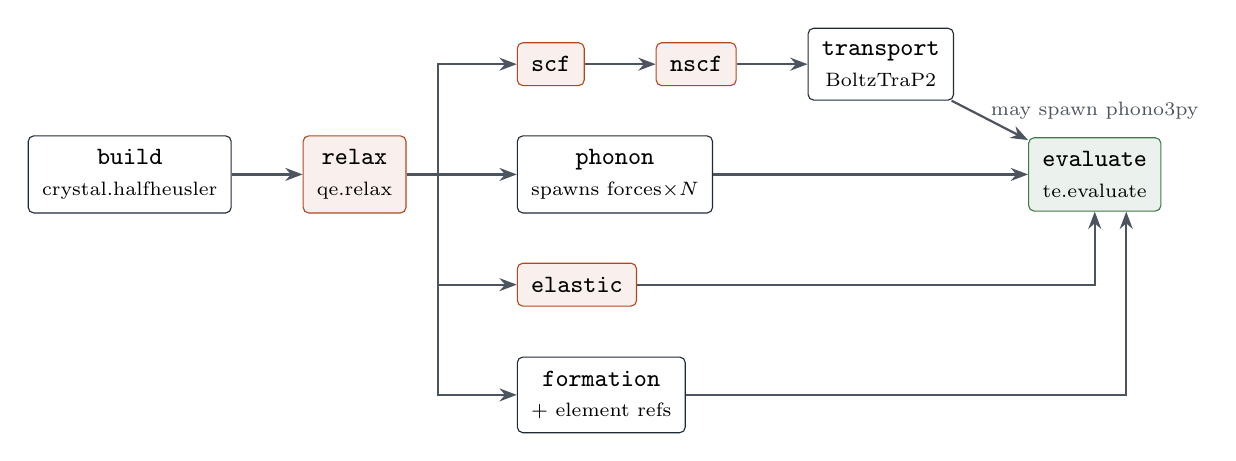
\begin{tikzpicture}[node distance=6mm and 9mm,every node/.style={font=\small}]
\node[box] (build) {\code{build}\\\scriptsize crystal.halfheusler};
\node[fbox,right=of build] (relax) {\code{relax}\\\scriptsize qe.relax};
\node[fbox,right=14mm of relax,yshift=14mm] (scf) {\code{scf}};
\node[fbox,right=of scf] (nscf) {\code{nscf}};
\node[box,right=of nscf] (tr) {\code{transport}\\\scriptsize BoltzTraP2};
\node[box,right=14mm of relax] (ph) {\code{phonon}\\\scriptsize spawns forces$\times N$};
\node[fbox,right=14mm of relax,yshift=-14mm] (el) {\code{elastic}};
\node[box,right=14mm of relax,yshift=-28mm] (form) {\code{formation}\\\scriptsize + element refs};
\node[mbox,right=40mm of ph] (ev) {\code{evaluate}\\\scriptsize te.evaluate};
\draw[arr] (build) -- (relax);
\draw[arr] (relax.east) -- ++(4mm,0) |- (scf);
\draw[arr] (relax) -- (ph);
\draw[arr] (relax.east) -- ++(4mm,0) |- (el);
\draw[arr] (relax.east) -- ++(4mm,0) |- (form);
\draw[arr] (scf) -- (nscf); \draw[arr] (nscf) -- (tr);
\draw[arr] (tr) -- (ev); \draw[arr] (ph) -- (ev);
\draw[arr] (el) -| (ev); \draw[arr] (form) -| ([xshift=4mm]ev.south);
\node[lab,above=1mm of ev] {may spawn phono3py};
\end{tikzpicture}
\caption{The per-material pipeline. Orange steps run DFT with Quantum ESPRESSO.}
\label{fig:pipeline}
\end{figure}

\begin{center}
\small
\begin{tabularx}{\linewidth}{@{}lXl@{}}
\toprule
Step & What it computes & Record kind \\
\midrule
\code{relax} & equilibrium structure and energy & \code{qe.relax} \\
\code{scf} & converged density & \code{qe.scf} \\
\code{nscf} & dense band structure, gap & \code{qe.bands} \\
\code{transport} & $S$, $\sigma/\tau$, $\ke$ vs.\ $T$ and doping & \code{transport.crta} \\
\code{phonon} & phonons, stability, $\gamma$, $\theta_D$, Slack $\kl$ & \code{phonon.harmonic}, \code{phonon.slack} \\
\code{elastic} & $C_{ij}$, Born stability, sound speeds & \code{stability.elastic} \\
\code{formation} & $E_f$, $E_\mathrm{hull}$ & \code{stability.formation} \\
\code{evaluate} & $ZT(T)$, screening verdict & \code{te.evaluate} \\
phono3py tier & BTE $\kl$, re-evaluated $ZT$ & \code{phonon.bte} \\
\code{validate} & comparison with literature & \code{te.validation} \\
\bottomrule
\end{tabularx}
\end{center}

\section{Screening}

A candidate passes screening when it is dynamically stable, Born stable,
$E_\mathrm{hull}\le0.1$\,eV/atom, has a band gap of at least 0.05\,eV, and reaches a peak $ZT$ of
at least 0.3 (with Slack $\kl$) for either carrier type. \code{te.evaluate} also attaches
practical scores (crustal abundance of the scarcest element, cost per kg, and toxicity) from
\code{data/elements.json}.

\section{Validation against experiment}

Before trusting the pipeline on unknown compounds, it is run on five known ones and compared with
published values (\code{data/literature\_halfheusler.json}, every value with a DOI). The checks:
\begin{itemize}
\item lattice constant within 2\% of experiment;
\item band gap within 0.2\,eV of published PBE values, with the right character (direct or indirect);
\item dynamically and mechanically stable, with negative formation energy;
\item Slack $\kl$ within a factor of 3 of experiment; phono3py $\kl$ for ZrNiSn within a factor of 1.5;
\item the ranking of $\kl$ matches experiment for most adjacent pairs, and the known best p- and
  n-type materials (NbFeSb, ZrNiSn) come out on top.
\end{itemize}
The literature values are also stored in the database as \code{LITERATURE} evidence, so the
dashboard shows predicted and measured values side by side. A miss is not hidden: the report
must explain it.

%======================================================================
\part{The distributed system}
%======================================================================

\chapter{Why a custom runtime}

Scientific clusters usually run Slurm, and cloud services run Kubernetes. Both assume dedicated,
administered machines. FireForge targets a looser setting: a handful of Linux workstations,
possibly in different places, some shared with people doing other work, joined over Tailscale.
The requirements were:
\begin{itemize}
\item install as an ordinary Linux service (\code{systemd}), with no cluster administrator;
\item strict per-node limits, so a workstation lent to the project keeps a share for its owner;
\item survive any machine or the coordinator restarting without losing or duplicating results;
\item move large result files directly between machines, not through a central server;
\item record where every number came from (provenance).
\end{itemize}
The result is \textbf{TDR}, built in nine phases. Each phase adds one capability on top of the
previous ones, and the chapters below follow that order.

\begin{figure}[h]
\centering
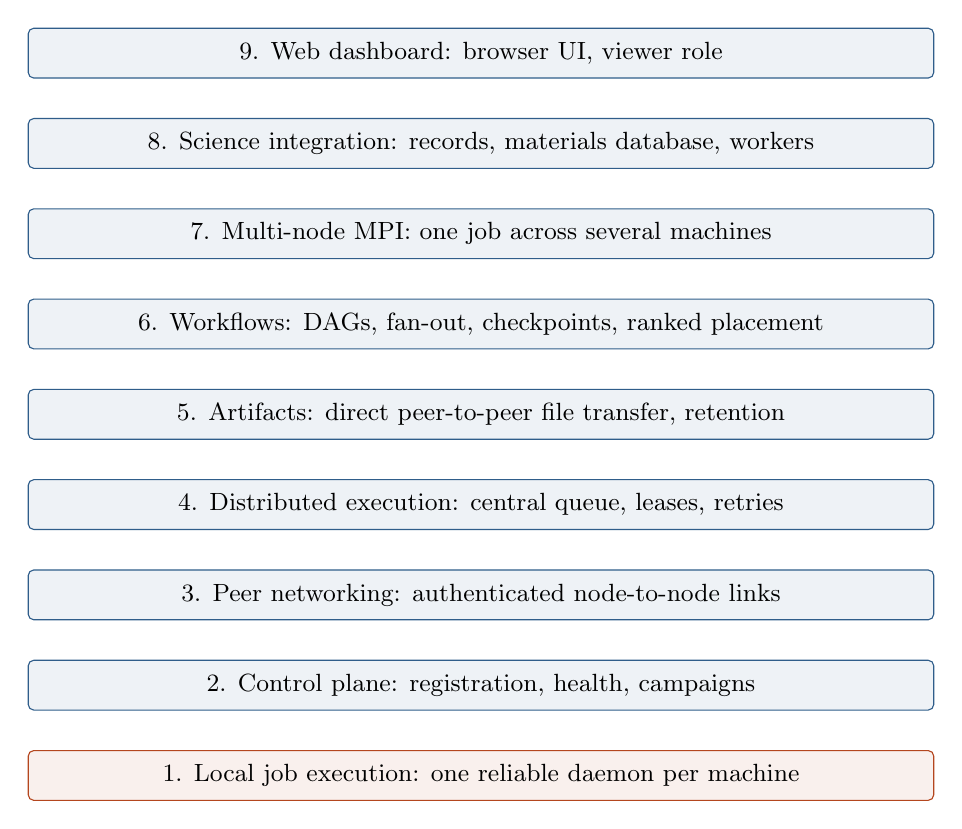
\begin{tikzpicture}[node distance=5mm]
\node[sbox,minimum width=11.5cm] (p9) {9. Web dashboard: browser UI, viewer role};
\node[sbox,minimum width=11.5cm,below=of p9] (p8) {8. Science integration: records, materials database, workers};
\node[sbox,minimum width=11.5cm,below=of p8] (p7) {7. Multi-node MPI: one job across several machines};
\node[sbox,minimum width=11.5cm,below=of p7] (p6) {6. Workflows: DAGs, fan-out, checkpoints, ranked placement};
\node[sbox,minimum width=11.5cm,below=of p6] (p5) {5. Artifacts: direct peer-to-peer file transfer, retention};
\node[sbox,minimum width=11.5cm,below=of p5] (p4) {4. Distributed execution: central queue, leases, retries};
\node[sbox,minimum width=11.5cm,below=of p4] (p3) {3. Peer networking: authenticated node-to-node links};
\node[sbox,minimum width=11.5cm,below=of p3] (p2) {2. Control plane: registration, health, campaigns};
\node[fbox,minimum width=11.5cm,below=of p2] (p1) {1. Local job execution: one reliable daemon per machine};
\end{tikzpicture}
\caption{The phases, each building on the ones below.}
\end{figure}

\chapter{Phase 1: running jobs reliably on one machine}

\section{The daemon and its parts}

Each machine runs \code{tdrd}, a long-lived daemon. You talk to it with \code{tdrctl} over a
Unix socket. Inside, it has a few modules:

\begin{description}
\item[JobManager] the job state machine: admission, attempts, retries, commit.
\item[Journal] an SQLite database recording every state change, so nothing is lost in a crash.
\item[ArtifactStore] a content-addressed file store (below).
\item[Supervisor] starts each job as an isolated child process with resource limits, and watches it.
\end{description}

The daemon is single-threaded: everything runs on one event loop (Boost.Asio), so no locks
are needed, and long work happens in child processes, not in the daemon.

\section{Jobs and their life cycle}

A \textbf{job} is one unit of work: a command to run, the resources it needs (cores, memory),
required capabilities (``needs QE''), input files, a timeout and a retry policy. Its life:

\begin{center}
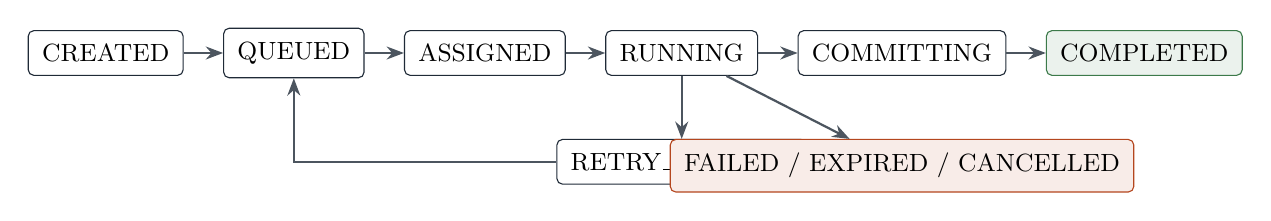
\begin{tikzpicture}[node distance=4mm and 5mm,every node/.style={font=\scriptsize}]
\node[box] (c) {CREATED}; \node[box,right=of c] (q) {QUEUED};
\node[box,right=of q] (a) {ASSIGNED}; \node[box,right=of a] (r) {RUNNING};
\node[box,right=of r] (cm) {COMMITTING}; \node[mbox,right=of cm] (ok) {COMPLETED};
\node[box,below=8mm of r] (rp) {RETRY\_PENDING};
\node[box,below=8mm of cm,fill=forge!10,draw=forge] (f) {FAILED / EXPIRED / CANCELLED};
\foreach \x/\y in {c/q,q/a,a/r,r/cm,cm/ok} \draw[arr] (\x)--(\y);
\draw[arr] (r) -- (rp); \draw[arr] (rp) -| (q); \draw[arr] (r) -- (f);
\end{tikzpicture}
\end{center}

Each try is an \textbf{attempt} with its own ID and its own scratch directory. A failed
attempt goes back to the queue if attempts remain. \textbf{Admission} is first-in first-out
within the node's caps: a job starts only when its cores and memory fit what is left.

\section{Running an attempt safely}

The supervisor launches the job's command as a child process and tracks it with a
\code{pidfd} (a race-free handle to a process). Limits come from \textbf{cgroups v2}, the Linux
kernel's resource-control mechanism (memory maximum, CPU quota). Where cgroups are not
available, it falls back to \code{setrlimit}, where the memory request becomes a cap on the
process's address space.

\begin{keyidea}[A lesson from the Phase 8 run]
That fallback once bit us: spawned science steps that did not request memory got the node's
64\,MB default, and numerical libraries failed to even load (``failed to map segment''). Every
science step now declares its memory (6\,GB for a screening QE step).
\end{keyidea}

A job writes outputs into its attempt directory. When it finishes, the daemon
\textbf{commits}: it checks the declared outputs exist, moves them into the artifact store and
records the result in the journal in one step. Either the whole result is published or none
of it is.

\section{Content-addressed artifacts}

Every output file becomes an \textbf{artifact}, named by the SHA-256 hash of its content:
\code{artifact://\allowbreak sha256/\allowbreak 9f2c\ldots}. Content addressing gives three properties for free:
identical files are stored once; a file can never change under its name; and anyone receiving
a file can verify it by re-hashing. Inputs to later jobs are referenced by these names.

\section{Crash recovery}

Because every state change is in the journal before it takes effect, a restarted daemon can
rebuild its state. It finds attempts that were running, checks whether their processes still
exist, and either reattaches or marks them for retry. Half-written outputs live in attempt
directories and are discarded; committed ones are in the store.

\section{The wire format}

Programs talk to the daemon (and later, daemons talk to each other) with a fixed binary
format: a 48-byte header followed by a Protocol Buffers payload.

\begin{center}
\small
\begin{tabular}{rrll}
\toprule
Offset & Size & Field & Notes\\
\midrule
0 & 4 & magic & \code{FFTR}\\
4 & 2 & version & 1\\
6 & 2 & message type & e.g.\ JOB\_SUBMIT, ARTIFACT\_REQUEST\\
8 & 4 & flags & 0\\
12 & 4 & payload length & at most 64 MiB\\
16 & 8 & message ID & \\
24 & 8 & correlation ID & the request's ID on a reply\\
32 & 16 & sender ID & node ID\\
\bottomrule
\end{tabular}
\end{center}

All integers are big-endian. \textbf{Protocol Buffers} (protobuf) is a schema language: message
types are defined once in \code{proto/} files and compiled into C++ and Python code, so both
sides agree on the format and new fields can be added without breaking old programs.

\section{Workers and the Python SDK}

A science job is a Python program using the SDK (\code{sdk/python/fireforge}). The daemon
passes the job a socket; the SDK connects, receives a \code{WorkerTask} (operation name,
parameters, input file paths, output directory) and sends back a \code{WorkerResult}. A worker
looks like this:

\begin{lstlisting}[language=Python]
@worker.task("qe.relax")
def relax(ctx):
    structure = load(ctx.input("structure"))
    result = engine.relax(structure, settings)       # runs pw.x
    ctx.save_output("structure", result.structure)
    ctx.record("qe.relax", structure=result.structure,
               properties={"energy_ev_per_atom": ..., "a_angstrom": ...})
\end{lstlisting}

\chapter{Phase 2: the control plane}

\section{\code{tdrcp} and PostgreSQL}

The control plane, \code{tdrcp}, is a C++ HTTPS server backed by PostgreSQL. In Phase 2 it
tracks nodes and campaigns; later phases add the job queue, workflows and the materials
database. Its API is REST: JSON over HTTPS (\code{GET /api/v1/nodes}, \code{POST
/api/v1/workflows}, and so on). The JSON is generated from the same protobuf schemas, so one
definition serves C++, Python and the wire.

\section{Identity: a private certificate authority}

Every participant proves who it is with a TLS certificate signed by FireForge's own
\textbf{certificate authority} (CA). Both sides of each connection present certificates
(\textbf{mutual TLS}, mTLS). There are no passwords. The certificate's organisational-unit
field carries a \textbf{role}:

\begin{center}
\begin{tabular}{ll}
\toprule
Role & May do \\
\midrule
\code{node} & register, heartbeat, take leases, report job status \\
\code{admin} & everything an operator does: submit, cancel, set limits \\
\code{viewer} & read everything, change nothing (Phase 9) \\
\code{server} & identifies \code{tdrcp} itself to clients \\
\bottomrule
\end{tabular}
\end{center}

\code{tdrctl pki} issues certificates. The science cluster's PKI lives in
\code{\textasciitilde/.local/\allowbreak share/\allowbreak fireforge-sci/\allowbreak pki}.

\section{Registration, heartbeats and health}

When \code{tdrd} starts, it \textbf{registers}: it sends its hardware (cores, memory, GPUs),
software \textbf{capabilities} (detected ones like \code{cgroups} plus configured ones such as
\code{sci,qe,phonopy,phono3py,boltztrap2}) and network addresses. It then sends a
\textbf{heartbeat} every 10 seconds with its current load. The control plane marks a node STALE,
then OFFLINE, if heartbeats stop. Heartbeat replies carry the node's \textbf{policy}: limits an
admin set centrally (for example ``use at most 20 cores''), which the node applies live.

\section{Campaigns}

A \textbf{campaign} groups related work (``half-Heusler validation, QE''). Pausing a campaign
holds all its queued jobs; completing it closes it. Results carry their campaign, so the
database can be filtered by it.

\chapter{Phase 3: peer networking}

Nodes need to talk to each other directly, to transfer files and to coordinate multi-node jobs.
The control plane publishes a \textbf{peer directory} (each node's addresses), and every node keeps
a persistent TLS connection to every other online node, a full mesh. A dialler tries the LAN
address first and the Tailscale address second, checks the peer's certificate (only
\code{node} certificates are accepted, and the name must match the directory), and measures
round-trip time with pings. If a link drops it reconnects with backoff. Reachability is reported
to the control plane, which later uses it for placement.

\chapter{Phase 4: distributed execution}

\section{A central queue, pulled by nodes}

Jobs submitted to the control plane go into a central queue in PostgreSQL. Nodes \textbf{pull}:
whenever a node has spare capacity it asks for work (\code{POST /api/v1/leases}) and states how
many cores and how much memory it has free. The control plane hands out jobs that fit, whose
required capabilities the node has, and whose campaign is active. Pulling means a node never
receives work it cannot hold, and a busy or dead node simply stops asking.

\section{Leases and fencing}

Each handed-out job is a \textbf{lease}, valid for 60 seconds and renewed by every heartbeat. If
the node dies, heartbeats stop, the lease expires, the attempt is marked abandoned and the job is
queued again for another node.

That raises a classic distributed-systems problem: what if the ``dead'' node was only cut off,
and later comes back and reports a result for a job that has meanwhile been given to someone else?
The fix is a \textbf{fencing token}: a number that increases with every new attempt. Every status
report carries the token of the attempt it belongs to, and the control plane rejects reports
whose token is not current. A stale node can never overwrite the real result.

\begin{keyidea}[Exactly one result]
Leases plus fencing plus atomic commit mean each job ends with exactly one published result,
even if machines die, networks split, or the control plane restarts mid-job. On restart, the
control plane gives nodes one lease period of grace to renew before expiring anything.
\end{keyidea}

\section{The node side}

On the node, a \textbf{RemoteExecutor} turns each lease into an ordinary local job (Phase 1), and
listens to its state changes. Each change becomes a status update stored in a persistent
\textbf{outbox} and retried until the control plane acknowledges it, so updates survive daemon
restarts and network outages.

\chapter{Phase 5: moving data between machines}

A job's inputs are often another job's outputs, produced on a different machine. Phase 5 lets a
node fetch an artifact \textbf{directly from a peer} that holds it. The control plane only knows
\emph{where} copies are (\code{artifact\_locations}); payloads never pass through it.

\begin{itemize}
\item Transfers use a separate TLS data connection to the peer, are chunked, resumable after an
  interruption, optionally rate-limited, and verified by re-hashing at the end.
\item \textbf{Placement prefers holders}: a job waits up to 15 seconds (\code{locality\_wait})
  for a node that already has its inputs, then goes to anyone, who fetches them.
\item \textbf{Retention}: each node keeps its store under a disk cap and evicts least-recently-used
  artifacts, but never the last copy anywhere. Admins can pin artifacts to keep them.
\end{itemize}

\chapter{Phase 6: workflows}

\section{DAGs}

A scientific result needs many jobs in a particular order. A \textbf{workflow} is a directed
acyclic graph (DAG) of \textbf{steps}. Each step is a job template plus the steps it depends on and
which of their outputs it takes as inputs. The workflow engine lives in the control plane: when a
step's job finishes, in the same database transaction, it checks which waiting steps are now
ready, wires the parents' output artifacts into the children's inputs, and queues their jobs.

Steps have \textbf{run rules}: run if all dependencies succeeded (default), if any failed (cleanup),
or always (\code{validate} uses ``always'', so a report is written even when some compounds fail).
A step whose rule is not met is SKIPPED.

\section{Dynamic fan-out}

Sometimes the number of jobs is only known at run time: how many displaced supercells a phonon
calculation needs depends on the crystal's symmetry. A running step can therefore \textbf{spawn}
new steps into its own workflow (\code{ctx.spawn(...)}). Spawned steps are named
\code{<parent>/<name>}, for example \code{ZrNiSn.phonon/v0.d001} (volume 0, displacement 1). A step
that depends on the spawning step waits for the whole spawned subtree to finish.

\section{Checkpoints}

A long step can save its progress with \code{ctx.checkpoint(...)}. The checkpoint is stored as an
artifact and copied to a nearby peer. If the attempt dies, the retry, on any node, receives the
latest checkpoint and resumes instead of starting again.

\section{Ranked placement}

Some jobs care a lot about where they run (big inputs, scarce capabilities). The control plane
scores nodes by compute fit, data-transfer cost, queue length, memory headroom and contention, and
can \textbf{reserve} a job for its best-ranked node for a short window before offering it to the
next.

\chapter{Phase 7: one job across several machines}

Very large calculations use MPI, where one program runs as many cooperating processes
(\textbf{ranks}) that exchange messages. Phase 7 lets one job span several nodes as a
\textbf{gang}. The control plane reserves capacity on all chosen nodes and \textbf{drains} them until
every member is free, then leases the whole gang at once. The head node runs \code{mpirun}, whose
remote-launch hook is TDR's own \code{tdr-launch agent}, so every rank runs inside its node's
sandbox and limits, without ssh or Slurm. If any member is lost, the whole gang attempt fails and
is retried as a unit from the latest checkpoint.

\begin{inff}
The half-Heusler cells have only three atoms, so a single node is plenty and the Phase 8 run
does not use gangs. They matter for larger cells later.
\end{inff}

\chapter{Phase 8: wiring in the science}

\section{Records: from a worker to the database}

Files are fine for raw data, but you want to \emph{query} results: ``all compounds with
$ZT>0.5$''. Phase 8 adds \textbf{calculation records}. A worker attaches records to its result with
\code{ctx.record(kind, structure=..., properties=..., method=...)}, and they travel with the result:

\begin{center}
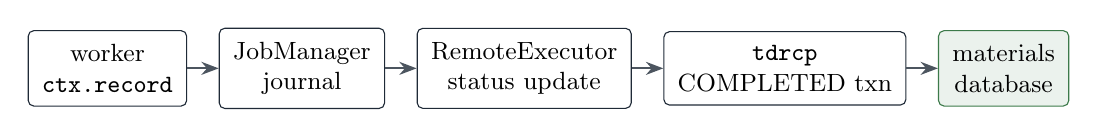
\begin{tikzpicture}[node distance=4mm,every node/.style={font=\scriptsize}]
\node[box] (w) {worker\\\code{ctx.record}};
\node[box,right=of w] (j) {JobManager\\journal};
\node[box,right=of j] (re) {RemoteExecutor\\status update};
\node[box,right=of re] (cp) {\code{tdrcp}\\COMPLETED txn};
\node[mbox,right=of cp] (db) {materials\\database};
\foreach \a/\b in {w/j,j/re,re/cp,cp/db} \draw[arr] (\a)--(\b);
\end{tikzpicture}
\end{center}

The control plane stores records in the \emph{same transaction} that marks the job completed, and
fencing applies, so a retried attempt can never add duplicates. Records are validated (at most 64
per job and 256\,KiB); invalid ones fail the job permanently.

\section{The materials database}

Three tables:
\begin{description}
\item[materials] one row per reduced formula (ZrNiSn), with its elements.
\item[structures] one row per distinct crystal (deduplicated by fingerprint), linked to its
  material, the job that produced it, and its parent structure.
\item[calculations] one row per record: kind, properties (JSON), conditions, method (solver,
  version, functional, pseudopotentials with checksums, settings), evidence (PREDICTED,
  LITERATURE or MEASURED), the output artifacts holding raw data, and full provenance: job,
  attempt, workflow, step, campaign and node.
\end{description}
Any number shown anywhere can be traced back to the exact calculation, settings and machine
that produced it.

\section{The science worker and workflow builders}

All science operations live in one worker program, \code{fireforge\_science.ops}, which dispatches
on the job's \code{operation}. Each node has a wrapper called \code{fireforge-sci} that runs it with
the right Python environment, so workflows can say \code{argv: ["fireforge-sci"]} and run on any
science node. Workflows are built in Python (\code{workflows.py}) and submitted as JSON:

\begin{lstlisting}
python -m fireforge_science submit-validation -o val.json
python -m fireforge_science submit-campaign --x Zr,Hf,Ti --y Ni,Co --z Sn,Sb -o hh.json
tdrctl cp workflow-submit val.json
\end{lstlisting}

A \code{toy} engine, a fast analytic stand-in for QE, lets the whole pipeline run in about two
minutes for tests. Its results are always labelled \code{engine: toy} and validation refuses them.

\chapter{Phase 9: the web dashboard}

\code{tdrcp} also serves a browser UI at \code{https://<control-plane>:8443/ui/}. The pages are
plain JavaScript compiled into the \code{tdrcp} binary; the browser reads the same REST API as
\code{tdrctl}. Login uses the same certificates: you import a \code{.p12} file (certificate plus key)
into the browser once. A \code{viewer} certificate sees everything and changes nothing; an
\code{admin} certificate also gets buttons to cancel jobs and workflows, pause campaigns, and set
node limits.

Because certificates are sent automatically, like cookies, the server guards against cross-site
request forgery: a state-changing request from a browser must come from the dashboard's own origin
and carry a JSON body. A strict Content Security Policy forbids any script or style not served by
\code{tdrcp} itself.

%======================================================================
\part{Putting it together}
%======================================================================

\chapter{Following ZrNiSn through the live system}

This is the validation workflow \code{wf-e3988d44d56f0017}, started on 6 November 2026.

\section{Submission}

The workflow was built with \code{validation\_workflow(engine="qe", preset="screening", cpus=4)}
and submitted with \code{sci-ctl workflow-submit}. It has 64 static steps:
\begin{itemize}
\item 18 for the nine elements (Co, Fe, Hf, Nb, Ni, Sb, Sn, Ti, Zr): \code{ref.El} builds the
  standard crystal of each element, \code{refrelax.El} relaxes it;
\item 9 per compound $\times$ 5 compounds = 45: build, relax, formation, scf, nscf, transport,
  phonon, elastic, evaluate;
\item 1 final \code{validate}.
\end{itemize}
More steps appear as phonon and phono3py steps spawn their force calculations.

\section{A relaxation, step by step}

\begin{enumerate}
\item \code{ZrNiSn.build} runs first (no dependencies): a light Python job that writes the
  half-Heusler structure with Ni on 4c. It completes in seconds; its output becomes an artifact
  on the HP.
\item The engine sees \code{ZrNiSn.relax} is now ready and queues its job: 4 cores, 6\,GB,
  capabilities \code{sci, qe}, input = the build artifact.
\item The HP's RemoteExecutor, which polls every few seconds while it has room, asks for a lease
  saying ``20 cores free'' (say) and receives this job with a fencing token.
\item \code{tdrd} starts \code{fireforge-sci} in a fresh attempt directory with a cgroup limited
  to 4 cores and 6\,GB. The worker writes a \code{pw.in}, runs \code{mpirun -np 4 pw.x}, and parses
  the result: three relaxation steps, $a=6.150$\,\AA, about 10 minutes.
\item The worker saves outputs (\code{structure}, \code{energy}, \code{log}) and a \code{qe.relax}
  record. \code{tdrd} commits them, and the RemoteExecutor reports COMPLETED with the token,
  output artifact IDs and the record.
\item In one transaction \code{tdrcp} marks the job completed, stores the record (creating the
  structure and linking it to the ZrNiSn material), and queues the four steps waiting for the
  relaxed structure: scf, phonon, elastic and (once every compound and element has relaxed)
  formation.
\end{enumerate}

With 20 cores and 4 per QE step, five DFT calculations run at once. The light steps (1--2
cores) fill in the gaps.

\section{What happens next}

\code{ZrNiSn.phonon} spawns its displaced-supercell force jobs at three volumes plus a collect
step; the transport branch runs scf, nscf and BoltzTraP2; elastic runs its strains with
checkpoints. When all branches are done, \code{ZrNiSn.evaluate} computes $ZT$ with Slack $\kl$ and,
because the tier is forced for ZrNiSn, spawns the phono3py steps: several hundred force
calculations, the longest part of the whole run. Finally \code{validate} compares every compound
with the literature and writes \code{report.md}, \code{report.json} and \code{te.validation}
records.

\section{Watching it}

\begin{itemize}
\item \textbf{Dashboard} (\code{https://<control-plane>:8443/}): Workflows shows the step graph live,
  Materials shows each compound with predicted-versus-literature checks and $ZT$ curves as results
  land, Results ranks all evaluated compounds.
\item \textbf{Command line}:
\begin{lstlisting}
S=~/.local/share/fireforge-sci
$S/sci-ctl workflow wf-e3988d44d56f0017       # step states
$S/sci-ctl nodes                              # node health and load
$S/sci-ctl calcs --kind te.evaluate           # results
$S/sci-ctl material <material-id>             # one compound, latest per kind
\end{lstlisting}
\end{itemize}

\chapter{Where things live}

\section{Repository}

\begin{center}
\small
\begin{tabularx}{\linewidth}{@{}lX@{}}
\toprule
Path & Contents \\
\midrule
\code{runtime/} & C++ node runtime: jobs, journal, artifacts, supervisor, peer links, transfer, remote execution, gangs, \code{tdrd}, \code{tdrctl} \\
\code{control/} & \code{tdrcp}: database repository, API handlers, server, web dashboard (\code{control/ui}) \\
\code{proto/} & protobuf schemas shared by C++, Python and the wire \\
\code{sdk/python/fireforge/} & worker SDK \\
\code{science/fireforge\_science/} & physics: engines, operations, workflows, literature data \\
\code{docs/design/phase*.md} & design of each phase, with implementation notes \\
\code{tests/e2e/} & end-to-end tests on real daemons \\
\code{tools/} & build, test and setup scripts, all run under the memory cap \\
\bottomrule
\end{tabularx}
\end{center}

\section{On the machines}

\begin{center}
\small
\begin{tabularx}{\linewidth}{@{}lX@{}}
\toprule
Where & What \\
\midrule
control plane & service \code{fireforge-sci-tdrcp}; config and binaries in \code{\textasciitilde/.local/share/fireforge-sci}; database \code{fireforge\_sci} in \code{build/pg} \\
compute node & service \code{fireforge-sci-tdrd}; config \code{tdr.conf}; artifacts under \code{node/artifacts}; code in \code{\textasciitilde/fireforge} with its own virtual environment \\
browser access & \code{\textasciitilde/.local/share/fireforge-sci/browser/}: \code{viewer.p12}, \code{admin.p12}, CA certificate \\
\bottomrule
\end{tabularx}
\end{center}

\section{Development rules}

All builds and tests go through \code{tools/capped}, which puts them in one shared memory-limited
cgroup (8\,GB, 4 cores) so parallel work never starves the machine:
\begin{lstlisting}
tools/build.sh -B build/dev --test        # C++ build and unit tests
tools/pytest.sh science/tests             # science tests
tools/e2e.sh -k science                   # end-to-end tests
\end{lstlisting}

%======================================================================
\appendix
\chapter{Glossary}

\begin{description}[style=nextline,leftmargin=1.2cm]
\item[Artifact] An immutable file named by the SHA-256 hash of its content.
\item[Attempt] One try at running a job, with its own ID and fencing token.
\item[Band gap] Energy between the top of the valence band and the bottom of the conduction band.
\item[BoltzTraP2] Code that computes electronic transport from DFT bands.
\item[Brillouin zone] The set of distinct electron (or phonon) wave vectors in a crystal.
\item[Campaign] A named group of related jobs and results.
\item[Capability] A label a node advertises (\code{qe}, \code{phonopy}) and a job can require.
\item[Checkpoint] Saved progress of a running step, used to resume a retry.
\item[Control plane] \code{tdrcp}: the coordinator holding queue, workflows and database.
\item[Convex hull] Lower envelope of formation energies; phases above it are unstable.
\item[CRTA] Constant relaxation time approximation: one scattering time for all electrons.
\item[DFT] Density functional theory: quantum mechanics via the electron density.
\item[Fencing token] Increasing attempt number that makes stale result reports rejectable.
\item[Fingerprint] Hash of a symmetry-standardised structure; equal fingerprints mean the same crystal.
\item[Force constants] Second (or third) derivatives of energy with respect to atomic displacements.
\item[Grüneisen parameter $\gamma$] How phonon frequencies change with volume; measures anharmonicity.
\item[Half-Heusler] $XYZ$ compound in space group $F\bar43m$ with one empty sublattice.
\item[$\kl$, $\ke$] Lattice and electronic thermal conductivity.
\item[Lease] Time-limited permission for a node to run a job attempt, renewed by heartbeats.
\item[mTLS] Mutual TLS: both client and server prove identity with certificates.
\item[PBE] The exchange--correlation approximation used here; underestimates band gaps.
\item[Phonon] A quantised lattice vibration; carries heat.
\item[Power factor] $S^2\sigma$.
\item[Pseudopotential] Smooth effective potential replacing a nucleus and its core electrons.
\item[Record] A structured result (kind, properties, method, provenance) stored in the database.
\item[Seebeck coefficient $S$] Voltage per kelvin of temperature difference.
\item[Slack model] Closed-form estimate of $\kl$ from phonon properties.
\item[Spawn] A running step adding new steps to its own workflow.
\item[Supercell] Unit cell repeated several times, used for phonon calculations.
\item[TDR] FireForge's distributed execution runtime.
\item[Workflow] A DAG of steps run by the control plane.
\item[$ZT$] Thermoelectric figure of merit, $S^2\sigma T/(\ke+\kl)$.
\end{description}

\chapter{Units used in records}

\begin{center}
\small
\begin{tabular}{lll}
\toprule
Key suffix & Unit & Meaning \\
\midrule
\code{\_ev}, \code{\_ev\_per\_atom} & eV & energy (1 eV $\approx$ 96.5 kJ/mol) \\
\code{\_angstrom} & \AA & length, $10^{-10}$\,m \\
\code{\_thz} & THz & phonon frequency \\
\code{\_k} & K & temperature \\
\code{\_gpa} & GPa & elastic modulus \\
\code{\_w\_mk} & W\,m$^{-1}$K$^{-1}$ & thermal conductivity \\
\code{\_uv\_k} & \si{\micro\volt\per\kelvin} & Seebeck coefficient \\
\code{\_uw\_cmk2} & \si{\micro\watt\per\centi\metre\per\kelvin\squared} & power factor \\
\code{\_cm3} & cm$^{-3}$ & carrier concentration \\
\code{\_s} & s & time (e.g.\ relaxation time $\tau$) \\
\bottomrule
\end{tabular}
\end{center}

\end{document}
